\documentclass[11pt,a4paper]{article}

% --- Core IEEE Formatting & Fonts ---
\usepackage[utf8]{inputenc}
\usepackage[margin=1in]{geometry}

% Times New Roman for Body, Helvetica/Arial for Headings (Standard IEEE SRS font combo)
\usepackage{mathptmx} % Times New Roman
\usepackage[scaled=0.92]{helvet} % Helvetica/Arial

\usepackage{microtype}
\usepackage{setspace}
\onehalfspacing

\usepackage{xcolor}
\usepackage{graphicx}
\usepackage{booktabs}
\usepackage{tabularx}
\usepackage{longtable}
\usepackage{array}
\usepackage{enumitem}
\setlist{leftmargin=*,itemsep=2pt,topsep=3pt}

% Table of Contents with Dot Leaders
\usepackage{tocloft}
\renewcommand{\cftsecleader}{\cftdotfill{\cftdotsep}}

% --- Section Heading Formatting (IEEE Black & Clean Alignment) ---
\usepackage{titlesec}
\titleformat{\section}{\fontfamily{phv}\selectfont\Large\bfseries}{\thesection}{0.8em}{}
\titleformat{\subsection}{\fontfamily{phv}\selectfont\large\bfseries}{\thesubsection}{0.8em}{}
\titleformat{\subsubsection}{\fontfamily{phv}\selectfont\normalsize\bfseries\itshape}{\thesubsubsection}{0.8em}{}

% --- Running Headers & Footers (Exact Match to Template PDF) ---
\usepackage{fancyhdr}
\pagestyle{fancy}
\fancyhf{}
\lhead{\small \itshape Software Requirements Specification for LifeOS}
\rhead{\small \itshape Page \thepage}
\renewcommand{\headrulewidth}{0pt}
\renewcommand{\footrulewidth}{0pt}

% --- Hyperlinks (Clean IEEE Black/Dark Blue) ---
\usepackage{hyperref}
\hypersetup{
    colorlinks=true,
    linkcolor=black,
    filecolor=black,
    urlcolor=black,
    citecolor=black,
    pdftitle={Software Requirements Specification for LifeOS},
    pdfauthor={LifeOS Software Engineering Team}
}

% --- Code Listings ---
\usepackage{listings}
\lstset{
    basicstyle=\ttfamily\small,
    breaklines=true,
    captionpos=b,
    frame=single,
    showstringspaces=false,
    tabsize=2
}

% --- TikZ Diagrams ---
\usepackage{tikz}
\usetikzlibrary{shapes.geometric, arrows.meta, positioning, shadows, fit, backgrounds}

\begin{document}

% ==========================================
% COVER PAGE (Exact Alignment with Template PDF Page 1)
% ==========================================
\begin{titlepage}
    \thispagestyle{empty}
    
    % Top Thick Rule
    \noindent\rule{\linewidth}{2.5pt} \\[1.8cm]
    
    % Right-Aligned Title Block (Matching srs doc template.pdf layout)
    \begin{flushright}
        {\fontsize{32pt}{38pt}\fontfamily{phv}\selectfont\bfseries Software Requirements\\[0.2cm] Specification} \\[1.2cm]
        
        {\fontsize{20pt}{24pt}\fontfamily{phv}\selectfont for} \\[1.2cm]
        
        {\fontsize{32pt}{36pt}\fontfamily{phv}\selectfont\bfseries LifeOS} \\[0.3cm]
        {\fontsize{15pt}{19pt}\fontfamily{phv}\selectfont\itshape An AI-Orchestrated Personal Productivity Substrate} \\[1.2cm]
        
        {\fontsize{15pt}{19pt}\fontfamily{phv}\selectfont\bfseries Version 1.0 approved} \\[1.2cm]
        
        {\fontsize{14pt}{18pt}\fontfamily{phv}\selectfont\bfseries Prepared by \\
        24BCE1622 - Abhinava Kasavajhala\\ 
        24BCE5339 - Parth Pareek \\
        24BCE5374 - Jahaan Suthar \\ 
        } \\[0.6cm]
        
        {\fontsize{14pt}{18pt}\fontfamily{phv}\selectfont LifeOS Platform Organization} \\[0.5cm]
        
        {\fontsize{14pt}{18pt}\fontfamily{phv}\selectfont July 22, 2026}
    \end{flushright}
    
    \vfill
    
\end{titlepage}

\newpage
\pagenumbering{roman}
\setcounter{page}{2}

% ==========================================
% PAGE ii: TABLE OF CONTENTS & REVISION HISTORY (Exact Match to Template PDF Page 2)
% ==========================================
\noindent {\fontfamily{phv}\selectfont\Huge\bfseries Table of Contents} \\[0.5cm]

\tableofcontents

\vspace{1cm}

\noindent {\fontfamily{phv}\selectfont\Huge\bfseries Revision History} \\[0.5cm]

\begin{table}[h!]
\centering
\begin{tabularx}{\textwidth}{|X|l|X|l|}
\hline
\textbf{Name} & \textbf{Date} & \textbf{Reason For Changes} & \textbf{Version} \\ \hline
Systems Architect & 2026-07-10 & Initial Vision and Architectural Boundary Outline & 0.1 \\ \hline
Lead Backend Engineer & 2026-07-14 & Modular Monolith \& AI Gateway Technical Specifications & 0.4 \\ \hline
AI Systems Lead & 2026-07-17 & CrewAI Multi-Agent Workflows \& Long-Term Memory Specs & 0.7 \\ \hline
Systems Architect & 2026-07-20 & Non-Functional Requirements \& Security Protocol Baseline & 0.9 \\ \hline
LifeOS Core Team & 2026-07-22 & Final Production Specification Release (IEEE 830 Format) & 1.0 \\ \hline
\end{tabularx}
\end{table}

\newpage
\pagenumbering{arabic}
\setcounter{page}{1}

% ==========================================
% 1. INTRODUCTION (Template PDF Page 3)
% ==========================================
\section{Introduction}

\subsection{Purpose}
Identify the product whose software requirements are specified in this document, including the revision or release number. Describe the scope of the product that is covered by this SRS, particularly if this SRS describes only part of the system or a single subsystem.

This Software Requirements Specification (SRS) document details the complete functional, non-functional, external interface, architectural, and operational requirements for the \textbf{LifeOS Platform (Version 1.0 approved)}. LifeOS is an AI-powered personal life management platform built as a cross-platform React Native mobile application, backed by a NestJS modular monolith backend and a Python CrewAI orchestration service. This specification encompasses the scope of the full production platform, including identity management, intelligent daily planning, Markdown notes, receipt OCR expense tracking, document vault storage, study tools, vector-based long-term memory, universal hybrid search, and Google Workspace integrations.

This document serves as the primary technical specification for software developers, system architects, database administrators, QA automation engineers, and project managers throughout the software development lifecycle.

\subsection{Document Conventions}
Describe any standards or typographical conventions that were followed when writing this SRS, such as fonts or highlighting that have special significance. For example, state whether priorities for higher-level requirements are assumed to be inherited by detailed requirements, or whether every requirement statement is to have its own priority.

This document strictly adheres to the \textbf{IEEE Std 830-1998 Standard for Software Requirements Specifications}.
\begin{itemize}
    \item \textbf{Typography:} Section headings use Helvetica/Arial bold fonts; body text is rendered in 11pt Times New Roman with 1-inch margins. Technical symbols, database models, and API paths are formatted in \texttt{monospace} font.
    \item \textbf{Requirement Tagging:} Functional requirements within Section 4 are uniquely identified with a sequence tag matching the format \texttt{REQ-[MODULE]-[NUMBER]} (for example, \texttt{REQ-AUTH-1}, \texttt{REQ-PLAN-1}, \texttt{REQ-AIGW-1}).
    \item \textbf{Priority Ratings:} Every detailed requirement statement specifies its own relative priority rating:
    \begin{itemize}
        \item \textbf{High:} Essential requirement mandatory for system operation and launch.
        \item \textbf{Medium:} Important capability scheduled for primary release rollout.
        \item \textbf{Low:} Extended feature designed for post-launch iteration.
    \end{itemize}
\end{itemize}

\subsection{Intended Audience and Reading Suggestions}
Describe the different types of reader that the document is intended for, such as developers, project managers, marketing staff, users, testers, and documentation writers. Describe what the rest of this SRS contains and how it is organized. Suggest a sequence for reading the document, beginning with the overview sections and proceeding through the sections that are most pertinent to each reader type.

This SRS is structured for diverse technical and managerial stakeholders:
\begin{enumerate}
    \item \textbf{Frontend Mobile Developers:} Focus on Section 2.1, Section 3.1 (User Interfaces), Section 3.4 (Communications Interfaces), and Section 4 (System Features UI screens).
    \item \textbf{Backend Platform Engineers:} Focus on Section 2 (Overall Description), Section 3.3 (Software Interfaces), Section 4 (System Features), Section 5 (Other Nonfunctional Requirements), and Section 6 (Other Requirements: Database and API Schemas).
    \item \textbf{AI Orchestration \& ML Engineers:} Focus on Section 4.3 (AI Gateway \& Multi-Agent Orchestration), Section 4.9 (Long-Term Memory), Section 6, and Appendix B.
    \item \textbf{Quality Assurance \& Testers:} Utilize Section 4 stimulus/response sequences and Section 5 performance standards to build automated test suites.
\end{enumerate}

\subsection{Product Scope}
Provide a short description of the software being specified and its purpose, including relevant benefits, objectives, and goals. Relate the software to corporate goals or business strategies. If a separate vision and scope document is available, refer to it rather than duplicating its contents here.

LifeOS addresses the problem of digital fragmentation in personal productivity. Modern individuals manage their lives across fragmented, disconnected applications for task tracking, calendar scheduling, personal notes, expense tracking, flashcards, and file storage. LifeOS unifies these domains into a single intelligent substrate, acting as the user's digital \textbf{Second Brain}.

\textit{Core Product Vision Directive:} LifeOS should never feel like ten separate productivity apps. It should feel like one intelligent assistant that understands relationships between all of the user's information and helps them make better decisions every day.

\subsubsection{Scope Boundaries}
\begin{itemize}
    \item \textbf{In-Scope Capabilities:} Cross-platform React Native client (iOS/Android), NestJS Modular Monolith backend, embedded NestJS AI Gateway, Python CrewAI multi-agent service, bi-directional Google Workspace sync, vector embedding storage (\texttt{pgvector}), and hybrid search.
    \item \textbf{Out-of-Scope (Non-Goals):} Building a custom low-level operating system kernel/ROM, replacing raw Google storage hosting, or desktop native binaries for Phase 1.
\end{itemize}

\subsection{References}
List any other documents or Web addresses to which this SRS refers. These may include user interface style guides, contracts, standards, system requirements specifications, use case documents, or a vision and scope document. Provide enough information so that the reader could access a copy of each reference, including title, author, version number, date, and source or location.

\begin{enumerate}
    \item IEEE Computer Society, \textit{IEEE Std 830-1998: IEEE Recommended Practice for Software Requirements Specifications}, IEEE, 1998.
    \item Karl E. Wiegers, \textit{Software Requirements}, 2nd Edition, Microsoft Press, 2003.
    \item NestJS Documentation, \textit{Modular Monolith Architecture \& Patterns}, \url{https://docs.nestjs.com/}.
    \item CrewAI Framework Specifications, \textit{Multi-Agent Collaboration Engine}, \url{https://docs.crewai.com/}.
    \item PostgreSQL Global Development Group, \textit{PostgreSQL 15 Relational Database \& pgvector Reference}, 2023.
    \item Google Workspace API Reference, \textit{OAuth 2.0 and REST Integration Standards}, Google Developers, 2025.
\end{enumerate}

\newpage
% ==========================================
% 2. OVERALL DESCRIPTION (Template PDF Page 4)
% ==========================================
\section{Overall Description}

\subsection{Product Perspective}
Describe the context and origin of the product being specified in this SRS. For example, state whether this product is a follow-on member of a product family, a replacement for certain existing systems, or a new, self-contained product. If the SRS defines a component of a larger system, relate the requirements of the larger system to the functionality of this software and identify interfaces between the two. A simple diagram that shows the major components of the overall system, subsystem interconnections, and external interfaces can be helpful.

LifeOS is a new, self-contained product engineered as a multi-tier platform consisting of:
1. A \textbf{React Native Mobile Client} (Thin Client presentation layer).
2. A \textbf{NestJS Backend Server} (Modular Monolith owning database persistence and API routes).
3. An \textbf{AI Gateway Subsystem} (Embedded inside NestJS to control AI routing and context assembly).
4. A \textbf{CrewAI Service} (Independent Python microservice for multi-agent workflows).

The backend is structured as a Modular Monolith rather than microservices to eliminate unnecessary network overhead and distributed transaction complexity. The CrewAI Python service is strictly an AI reasoning layer; it has no direct database access and communicates exclusively with the NestJS AI Gateway via HTTP APIs.

\begin{figure}[h!]
\centering
\resizebox{\textwidth}{!}{
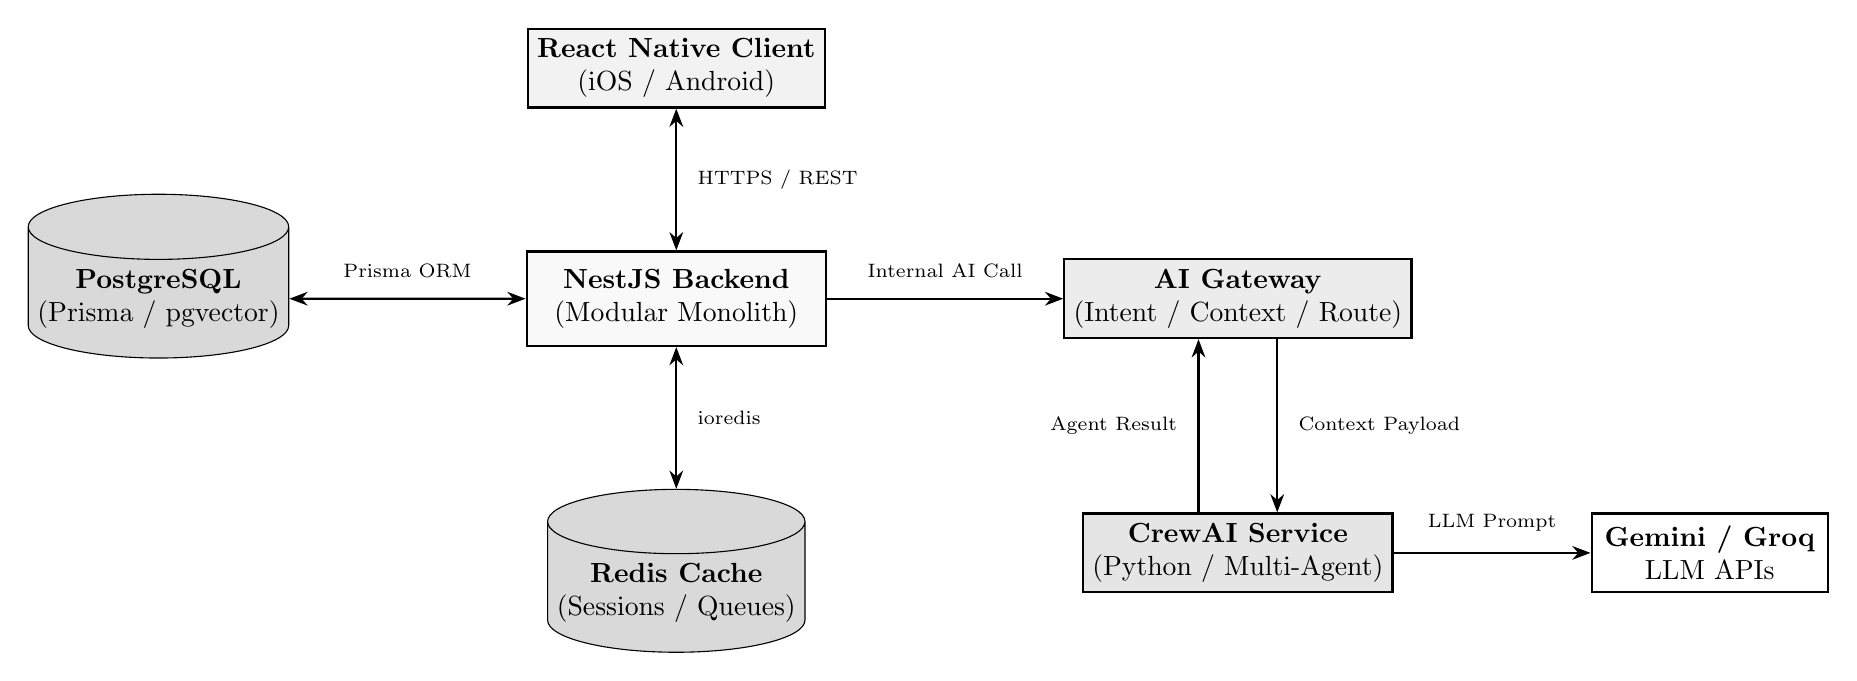
\begin{tikzpicture}[node distance=2.0cm, auto, >=Stealth]
    \tikzstyle{client} = [rectangle, draw=black, fill=gray!10, thick, minimum width=3.4cm, minimum height=1.0cm, align=center]
    \tikzstyle{backend} = [rectangle, draw=black, fill=gray!5, thick, minimum width=3.8cm, minimum height=1.2cm, align=center]
    \tikzstyle{gateway} = [rectangle, draw=black, fill=gray!15, thick, minimum width=3.8cm, minimum height=1.0cm, align=center]
    \tikzstyle{crew} = [rectangle, draw=black, fill=gray!20, thick, minimum width=3.4cm, minimum height=1.0cm, align=center]
    \tikzstyle{db} = [cylinder, draw=black, fill=gray!30, shape border rotate=90, aspect=0.25, minimum width=2.4cm, minimum height=1.2cm, align=center]
    \tikzstyle{llm} = [rectangle, draw=black, fill=white, thick, minimum width=3.0cm, minimum height=1.0cm, align=center]

    % Nodes with generous spacing
    \node (rn) [client] {\textbf{React Native Client}\\(iOS / Android)};
    \node (nest) [backend, below=1.8cm of rn] {\textbf{NestJS Backend}\\(Modular Monolith)};
    \node (pg) [db, left=3.0cm of nest] {\textbf{PostgreSQL}\\(Prisma / pgvector)};
    \node (redis) [db, below=1.8cm of nest] {\textbf{Redis Cache}\\(Sessions / Queues)};
    \node (gw) [gateway, right=3.0cm of nest] {\textbf{AI Gateway}\\(Intent / Context / Route)};
    \node (crew) [crew, below=2.2cm of gw] {\textbf{CrewAI Service}\\(Python / Multi-Agent)};
    \node (llm) [llm, right=2.5cm of crew] {\textbf{Gemini / Groq}\\LLM APIs};

    % Connections with clean offsets and font sizing
    \draw[<->, thick] (rn) -- node[right=4pt, font=\scriptsize] {HTTPS / REST} (nest);
    \draw[<->, thick] (nest) -- node[above=4pt, font=\scriptsize] {Prisma ORM} (pg);
    \draw[<->, thick] (nest) -- node[right=4pt, font=\scriptsize] {ioredis} (redis);
    \draw[->, thick] (nest) -- node[above=4pt, font=\scriptsize] {Internal AI Call} (gw);
    
    % Dual vertical arrows with clean horizontal shifts
    \draw[->, thick] ([xshift=0.5cm]gw.south) -- node[right=4pt, font=\scriptsize] {Context Payload} ([xshift=0.5cm]crew.north);
    \draw[<-, thick] ([xshift=-0.5cm]gw.south) -- node[left=4pt, font=\scriptsize] {Agent Result} ([xshift=-0.5cm]crew.north);
    
    \draw[->, thick] (crew) -- node[above=4pt, font=\scriptsize] {LLM Prompt} (llm);
\end{tikzpicture}
}
\caption{LifeOS System Architecture and Data Ownership Boundaries}
\label{fig:arch_diagram}
\end{figure}

\subsection{Product Functions}
Summarize the major functions the product must perform or must let the user perform. Details will be provided in Section 3, so only a high level summary (such as a bullet list) is needed here. Organize the functions to make them understandable to any reader of the SRS. A picture of the major groups of related requirements and how they relate, such as a top level data flow diagram or object class diagram, is often effective.

The major functions performed by LifeOS are organized into 11 functional domains:
\begin{enumerate}
    \item \textbf{Authentication \& Security:} Google OAuth2 SSO, email/password JWT tokens, refresh token rotation, and session revocation.
    \item \textbf{User Management:} Profile settings, global user preferences, currency standards, and GDPR account deletion.
    \item \textbf{AI Gateway Engine:} Prompt intent classification, database context collection, LLM routing (Gemini/Groq), and token audit logging.
    \item \textbf{Planner Engine:} Unified management of Google Calendar events, tasks (Eisenhower matrix), goals, and habit streak tracking.
    \item \textbf{Notes Vault:} Markdown rich text editing, automated AI summaries, tag indexing, and vector embedding generation.
    \item \textbf{Expense Engine:} Financial transaction ledger, vision-based receipt OCR extraction, AI category tagging, and budget analytics.
    \item \textbf{Document Vault:} PDF/Image file upload, cloud storage management, full-text extraction, and document indexing.
    \item \textbf{Study Hub:} Flashcard deck creation, AI quiz generation, and SuperMemo-2 (SM-2) spaced repetition engine.
    \item \textbf{Long-Term Memory Engine:} User-permissioned persistent vector memory, facts extraction, and memory audit control.
    \item \textbf{Universal Search Engine:} Reciprocal Rank Fusion (RRF) hybrid keyword and semantic vector search across all entities.
    \item \textbf{Google Workspace Sync:} Bi-directional synchronization for Calendar, Gmail receipts, Drive files, Contacts, and Photos.
\end{enumerate}

\subsection{User Classes and Characteristics}
Identify the various user classes that you anticipate will use this product. User classes may be differentiated based on frequency of use, subset of product functions used, technical expertise, security or privilege levels, educational level, or experience. Describe the pertinent characteristics of each user class. Certain requirements may pertain only to certain user classes. Distinguish the most important user classes for this product from those who are less important to satisfy.

\begin{itemize}
    \item \textbf{Academic Student (User Class 1):} High volume of notes, study decks, exam schedules, and daily budget limits. Relies on flashcard generation and schedule optimization. Technical expertise: Moderate.
    \item \textbf{Busy Professional (User Class 2):} Relies heavily on Google Calendar sync, automated schedule optimization, email receipt scanning, and fast meeting notes. Requires sub-second performance. Technical expertise: High.
    \item \textbf{Knowledge Creator (User Class 3):} Focuses on long-term memory synthesis, Markdown notes vault, document indexing, and habit tracking. Technical expertise: Moderate to High.
    \item \textbf{System Administrator (User Class 4):} Responsible for platform monitoring, LLM token budget management, circuit breaker tuning, and system audit logs. Technical expertise: Expert.
\end{itemize}

\subsection{Operating Environment}
Describe the environment in which the software will operate, including the hardware platform, operating system and versions, and any other software components or applications with which it must peacefully coexist.

\begin{enumerate}
    \item \textbf{Client Device Matrix:} Mobile OS: Apple iOS 15.0+ and Android 10.0+ (API Level 29+); Client Framework: React Native 0.73+ executing on Hermes engine.
    \item \textbf{Server Infrastructure Matrix:} Containerization: Docker 24.0+ managed via Docker Compose / Kubernetes; Application Runtime: Node.js v20.x LTS running NestJS 10.x; Database Engine: PostgreSQL 15.x with \texttt{pgvector} extension; Cache Store: Redis 7.x cluster; Python AI Service: Python 3.11 with FastAPI and CrewAI 0.28+.
\end{enumerate}

\subsection{Design and Implementation Constraints}
Describe any items or issues that will limit the options available to the developers. These might include: corporate or regulatory policies; hardware limitations (timing requirements, memory requirements); interfaces to other applications; specific technologies, tools, and databases to be used; parallel operations; language requirements; communications protocols; security considerations; design conventions or programming standards.

\begin{enumerate}
    \item \textbf{Backend-First Paradigm:} All validation, authorization, business rules, and state computations must occur inside NestJS. The React Native app is strictly a thin UI presentation layer.
    \item \textbf{Single Database Owner:} Only NestJS accesses PostgreSQL and Redis. The CrewAI Python service is strictly prohibited from opening direct database connections.
    \item \textbf{Single Gateway Entry Point:} All AI functionality must pass through the NestJS AI Gateway. Direct module-to-LLM calls are forbidden.
    \item \textbf{AI Non-Dependence:} Standard CRUD features (Notes, Tasks, Calendar, Expenses) must function perfectly as a traditional app if AI APIs are offline.
    \item \textbf{Deterministic Math Calculation:} Financial totals, budget sums, and calendar time overlap checks must be calculated in TypeScript, never delegated to an LLM.
\end{enumerate}

\subsection{User Documentation}
List the user documentation components (such as user manuals, on-line help, and tutorials) that will be delivered along with the software. Identify any known user documentation delivery formats or standards.

\begin{itemize}
    \item \textbf{Interactive In-App Onboarding:} Interactive walkthrough for new users demonstrating the 5 main tabs, Google account linking, and AI memory permissions.
    \item \textbf{In-App Help Center:} Searchable knowledge base covering features, privacy settings, and memory audit controls.
    \item \textbf{OpenAPI / Swagger Specs:} Interactive API specifications auto-generated at \texttt{/api/v1/docs}.
\end{itemize}

\subsection{Assumptions and Dependencies}
List any assumed factors (as opposed to known facts) that could affect the requirements stated in the SRS. These could include third-party or commercial components that you plan to use, issues around the development or operating environment, or constraints. The project could be affected if these assumptions are incorrect, are not shared, or change. Also identify any dependencies the project has on external factors, such as software components that you intend to reuse from another project, unless they are already documented elsewhere.

\begin{itemize}
    \item \textbf{Third-Party API Uptime:} Assumes $>99.9\%$ operational availability of Google Workspace APIs, Google Gemini API, and Groq Inference services.
    \item \textbf{Mobile Hardware Permissions:} Assumes users grant mobile device camera access for OCR scans and microphone access for voice input.
\end{itemize}

\newpage
% ==========================================
% 3. EXTERNAL INTERFACE REQUIREMENTS (Template PDF Page 5)
% ==========================================
\section{External Interface Requirements}

\subsection{User Interfaces}
Describe the logical characteristics of each interface between the software product and the users. This may include sample screen images, any GUI standards or product family style guides that are to be followed, screen layout constraints, standard buttons and functions that will appear on every screen, keyboard shortcuts, error message display standards, and so on. Define the software components for which a user interface is needed. Details of the user interface design should be documented in a separate user interface specification.

The LifeOS mobile user interface is organized around a \textbf{5-Tab Navigation Layout} engineered for ergonomics and speed.

\begin{figure}[h!]
\centering
\resizebox{\textwidth}{!}{
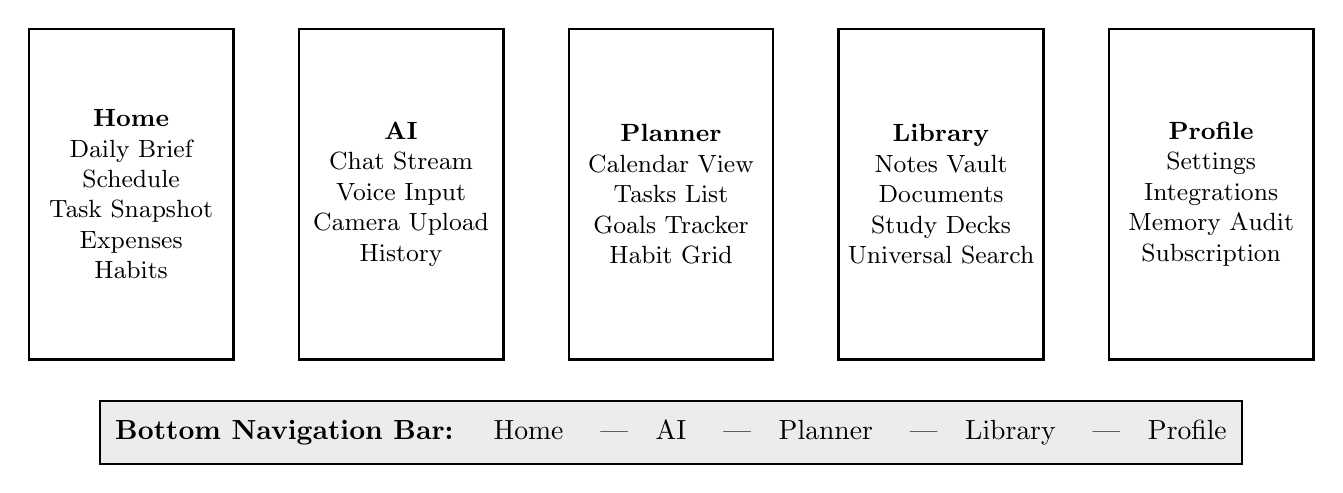
\begin{tikzpicture}[node distance=0.8cm]
    \tikzstyle{screen} = [rectangle, draw=black, fill=white, thick, minimum width=2.6cm, minimum height=4.2cm, align=center, font=\small]
    \tikzstyle{tabbar} = [rectangle, draw=black, fill=gray!15, thick, minimum width=14.5cm, minimum height=0.8cm, align=center]

    \node (s1) [screen] {\textbf{Home}\\Daily Brief\\Schedule\\Task Snapshot\\Expenses\\Habits};
    \node (s2) [screen, right=of s1] {\textbf{AI}\\Chat Stream\\Voice Input\\Camera Upload\\History};
    \node (s3) [screen, right=of s2] {\textbf{Planner}\\Calendar View\\Tasks List\\Goals Tracker\\Habit Grid};
    \node (s4) [screen, right=of s3] {\textbf{Library}\\Notes Vault\\Documents\\Study Decks\\Universal Search};
    \node (s5) [screen, right=of s4] {\textbf{Profile}\\Settings\\Integrations\\Memory Audit\\Subscription};

    \node (tb) [tabbar, below=0.5cm of s3] {\textbf{Bottom Navigation Bar:} \quad Home \quad|\quad AI \quad|\quad Planner \quad|\quad Library \quad|\quad Profile};
\end{tikzpicture}
}
\caption{LifeOS Client User Interface Navigation Structure}
\label{fig:ui_layout}
\end{figure}

\subsubsection{Detailed Screen Layouts}
\begin{enumerate}
    \item \textbf{Home Screen (\texttt{HomeScreen.tsx}):} Displays Daily Brief hero card, chronological event/task timeline, and snapshot widgets for budget, habits, and AI suggestions.
    \item \textbf{AI Screen (\texttt{AIScreen.tsx}):} Features full-duplex chat thread supporting Markdown and LaTeX rendering, voice waveform recording, camera image upload, and quick action chips.
    \item \textbf{Planner Screen (\texttt{PlannerScreen.tsx}):} Provides interactive month/week/day calendar, task lists with Eisenhower filtering, goal trackers, and habit streak grids.
    \item \textbf{Library Screen (\texttt{LibraryScreen.tsx}):} Contains folder/tag filtered notes vault, uploaded PDF document hub, study flashcard decks, and global search bar.
    \item \textbf{Profile Screen (\texttt{ProfileScreen.tsx}):} Manages Google integration toggles, memory audit vault (view/delete individual memories), subscription tier, and account settings.
\end{enumerate}

\subsection{Hardware Interfaces}
Describe the logical and physical characteristics of each interface between the software product and the hardware components of the system. This may include the supported device types, the nature of the data and control interactions between the software and the hardware, and communication protocols to be used.

\begin{itemize}
    \item \textbf{Camera Hardware Interface:} Accesses device camera for scanning paper receipts, document photos, and study notes (minimum 1080p resolution).
    \item \textbf{Microphone Hardware Interface:} Captures device audio hardware stream (16kHz mono PCM) for speech-to-text dictation.
    \item \textbf{Biometric Hardware Interface:} Interfaces with iOS FaceID/TouchID and Android BiometricPrompt for secure session locking.
\end{itemize}

\subsection{Software Interfaces}
Describe the connections between this product and other specific software components (name and version), including databases, operating systems, tools, libraries, and integrated commercial components. Identify the data items or messages coming into the system and going out and describe the purpose of each.

\begin{table}[h!]
\centering
\small
\begin{tabularx}{\textwidth}{|>{\raggedright\arraybackslash}p{3.0cm}|>{\raggedright\arraybackslash}p{2.5cm}|>{\raggedright\arraybackslash}p{2.5cm}|>{\raggedright\arraybackslash}X|}
\hline
\textbf{Software Component} & \textbf{Protocol / Driver} & \textbf{Data Format} & \textbf{Purpose} \\ \hline
PostgreSQL 15 & TCP / Prisma ORM & SQL Binary / JSONB & Primary persistent relational \& vector state storage \\ \hline
Redis 7 Cluster & TCP / ioredis & RESP Protocol & Cache, session store, rate limits, async queues \\ \hline
CrewAI Service & HTTP / REST API & JSON Payloads & Multi-agent workflow execution engine \\ \hline
Google OAuth2 & HTTPS / REST & JSON Web Tokens & Single Sign-On authentication \\ \hline
Google Calendar & HTTPS / REST & iCalendar JSON & Event synchronization \& time-blocking \\ \hline
Gmail API & HTTPS / REST & MIME / JSON DTOs & Parsing receipts, trip digests, \& reminders \\ \hline
Google Drive & HTTPS / REST & Binary PDF / JSON & Document ingestion \& storage backup \\ \hline
Google Photos & HTTPS / REST & Binary JPEG / Meta & Semantic photo search \& receipt lookup \\ \hline
Google Gemini / Groq & HTTPS / REST API & JSON Stream DTOs & High-speed \& complex reasoning LLM inference \\ \hline
\end{tabularx}
\caption{Software Interface Integration Matrix}
\end{table}

\subsection{Communications Interfaces}
Describe the requirements associated with any communications functions required by this product, including e-mail, web browser, network server communications protocols, electronic forms, and so on. Define any pertinent message formatting. Identify any communication standards that will be used, such as FTP or HTTP. Specify any communication security or encryption issues, data transfer rates, and synchronization mechanisms.

\begin{itemize}
    \item \textbf{Client-Server Communication:} RESTful API calls executed over \textbf{HTTPS} (TLS 1.3 encryption enforced). Real-time streaming AI responses utilize \textbf{WebSockets (WSS)} or Server-Sent Events.
    \item \textbf{Authentication Security:} HTTP Header: \texttt{Authorization: Bearer <JWT\_ACCESS\_TOKEN>}. Access Tokens expire in 15 minutes; Refresh Tokens stored in secure HTTP-only cookies expire in 7 days.
\end{itemize}

\newpage
% ==========================================
% 4. SYSTEM FEATURES (Template PDF Page 6)
% ==========================================
\section{System Features}

This section details the functional requirements organized by major system features.

% ----------------------------------------------------
\subsection{Authentication and Authorization Feature}
\subsubsection{Description and Priority}
Provides secure user login, Google OAuth2 SSO, email registration, password hashing, JWT token generation, refresh token rotation, and session management. \\
\textbf{Priority:} High.

\subsubsection{Stimulus/Response Sequences}
\begin{itemize}
    \item \textbf{User Action:} User taps "Sign in with Google" on the mobile login screen.
    \item \textbf{System Response:} Client opens Google OAuth2 PKCE web flow, captures auth code, posts code to NestJS backend, receives signed JWT access/refresh token pair, and loads Home Screen.
\end{itemize}

\subsubsection{Functional Requirements}
\begin{description}
    \item[REQ-AUTH-1:] The system shall authenticate users via Google OAuth2 authorization code flow with PKCE, validating ID token signatures on the backend before establishing a session.
    \item[REQ-AUTH-2:] The system shall support email and password registration and login. Passwords shall be hashed using Argon2id with 64MB memory cost and 3 iterations prior to storage.
    \item[REQ-AUTH-3:] The system shall issue 15-minute RS256-signed JWT access tokens and 7-day refresh tokens stored in Redis with single-use rotation enforcement.
    \item[REQ-AUTH-4:] Upon user logout, the system shall revoke the active refresh token in Redis and add the access token JTI to a Redis blacklist until token expiration.
\end{description}

% ----------------------------------------------------
\subsection{User Management and Profile Feature}
\subsubsection{Description and Priority}
Manages user profile details, application preferences, currency standards, and account teardown requests. \\
\textbf{Priority:} High.

\subsubsection{Stimulus/Response Sequences}
\begin{itemize}
    \item \textbf{User Action:} User updates display name and primary currency in Profile settings.
    \item \textbf{System Response:} Client submits PATCH request to backend, NestJS validates DTO, updates PostgreSQL record, and returns updated user profile object.
\end{itemize}

\subsubsection{Functional Requirements}
\begin{description}
    \item[REQ-USER-1:] The system shall allow users to view and edit profile details, including display name, avatar image URL, timezone, and primary currency code.
    \item[REQ-USER-2:] The system shall persist and synchronize user preferences (UI theme mode, notification time schedules, default calendar view) across client sessions.
    \item[REQ-USER-3:] Upon user request for account deletion, the backend shall perform a cascading delete purging all relational records, vectors, files, and cache entries within 24 hours.
\end{description}

% ----------------------------------------------------
\subsection{AI Gateway and Multi-Agent Orchestration Feature}
\subsubsection{Description and Priority}
Central intelligence middleware embedded inside NestJS. Intercepts AI requests, evaluates intent, builds database context, routes prompts to Python CrewAI or LLM providers (Gemini/Groq), logs token costs, and manages fallbacks. \\
\textbf{Priority:} High.

\subsubsection{Stimulus/Response Sequences}
\begin{itemize}
    \item \textbf{User Action:} User submits prompt "Organize my afternoon tasks and schedule them into calendar gaps".
    \item \textbf{System Response:} AI Gateway classifies intent as \texttt{INTENT\_PLAN\_SCHEDULE}, queries NestJS database for pending tasks and calendar events, packages context payload, routes request to CrewAI \texttt{PlannerCrew}, logs token usage, and streams optimized schedule to client UI.
\end{itemize}

\subsubsection{Functional Requirements}
\begin{description}
    \item[REQ-AIGW-1:] All AI requests from mobile screens or background schedule jobs shall pass strictly through the NestJS \texttt{AIGatewayService}. Direct calls to LLMs or CrewAI from domain modules are prohibited.
    \item[REQ-AIGW-2:] The AI Gateway shall classify incoming user prompts using a high-speed classifier model (Groq Llama-3-8B or Gemini Flash) into discrete intent categories: \texttt{PLAN\_DAY}, \texttt{ANALYZE\_EXPENSE}, \texttt{SUMMARIZE\_NOTE}, or \texttt{GENERAL\_CHAT}.
    \item[REQ-AIGW-3:] Upon intent classification, the AI Gateway shall fetch relevant context records from internal PostgreSQL repositories (tasks, events, memories) and format a structured context payload for the AI worker.
    \item[REQ-AIGW-4:] The Gateway shall dynamically select target models based on task complexity: simple summaries route to Groq/Gemini Flash; complex reasoning routes to Gemini Pro or CrewAI agent flows.
    \item[REQ-AIGW-5:] The AI Gateway shall log every execution to database table \texttt{AIUsageLog}, recording user ID, model, prompt tokens, completion tokens, execution latency (ms), and calculated monetary cost.
    \item[REQ-AIGW-6:] If a primary LLM provider fails or times out after 8 seconds, the Gateway circuit breaker shall automatically failover to a secondary model provider or return a graceful error message.
\end{description}

% ----------------------------------------------------
\subsection{Planner Feature (Calendar, Tasks, Goals, Habits)}
\subsubsection{Description and Priority}
Consolidates Google Calendar events, prioritized tasks (Eisenhower matrix), long-term goal milestones, and daily habit tracking. \\
\textbf{Priority:} High.

\subsubsection{Stimulus/Response Sequences}
\begin{itemize}
    \item \textbf{User Action:} User creates a new task titled "Prepare Presentation" with due date tomorrow.
    \item \textbf{System Response:} NestJS stores task in database, checks calendar for available focus time blocks, and highlights recommended time slots.
\end{itemize}

\subsubsection{Functional Requirements}
\begin{description}
    \item[REQ-PLAN-1:] The system shall provide full CRUD capabilities for calendar events, supporting title, start/end timestamps, location, RRULE recurrence parameters, and category color tags.
    \item[REQ-PLAN-2:] The system shall manage tasks with attributes including title, description, due date, estimated duration, priority level (Urgent/Important quadrant), and checklist items.
    \item[REQ-PLAN-3:] The system shall support defining long-term goals associated with target completion dates, categories, and progress percentage milestones.
    \item[REQ-PLAN-4:] The system shall track daily/weekly habits, recording completion timestamps, calculating active streak counts, longest streaks, and completion analytics.
    \item[REQ-PLAN-5:] The backend shall deterministically detect overlapping calendar events and time-blocked task allocations, returning warning payloads to the client UI.
    \item[REQ-PLAN-6:] Via the AI Gateway, the system shall analyze open calendar windows and pending tasks to propose an optimized daily time-blocked schedule.
\end{description}

% ----------------------------------------------------
\subsection{Notes and Knowledge Management Feature}
\subsubsection{Description and Priority}
Markdown note editor, AI note summarization, semantic tagging, and vector embedding indexing. \\
\textbf{Priority:} High.

\subsubsection{Stimulus/Response Sequences}
\begin{itemize}
    \item \textbf{User Action:} User saves a 1000-word lecture note in Markdown format.
    \item \textbf{System Response:} System saves note to PostgreSQL, triggers background job to generate 1536-dim vector embedding via \texttt{pgvector}, and generates 3-bullet AI summary.
\end{itemize}

\subsubsection{Functional Requirements}
\begin{description}
    \item[REQ-NOTE-1:] The system shall store structured Markdown notes supporting headers, code blocks, checklists, images, and custom category tags.
    \item[REQ-NOTE-2:] The system shall generate a concise 3-bullet AI summary for any note exceeding 500 words and store it in note metadata.
    \item[REQ-NOTE-3:] Upon saving any note, the backend shall generate text vector embeddings using \texttt{text-embedding-3-small} (1536 dimensions) and index them in PostgreSQL via \texttt{pgvector}.
\end{description}

% ----------------------------------------------------
\subsection{Expense Tracking and Receipt OCR Feature}
\subsubsection{Description and Priority}
Financial record keeping, manual expense entries, vision OCR receipt capture, AI category assignment, and budget analytics. \\
\textbf{Priority:} High.

\subsubsection{Stimulus/Response Sequences}
\begin{itemize}
    \item \textbf{User Action:} User takes photo of paper grocery receipt on mobile camera.
    \item \textbf{System Response:} System uploads photo, executes Google Vision API / Gemini Flash Vision OCR, extracts vendor, date, line items, total amount, creates draft expense record, and asks user to confirm.
\end{itemize}

\subsubsection{Functional Requirements}
\begin{description}
    \item[REQ-EXP-1:] The system shall record expenses with numeric transaction amount, date, vendor, category tag (Food, Transport, Utilities), payment method, and optional receipt image URL.
    \item[REQ-EXP-2:] The system shall process uploaded receipt images via Vision APIs to extract total cost, tax, vendor, date, and line items with $>90\%$ accuracy.
    \item[REQ-EXP-3:] All financial sums, category totals, and budget variance calculations shall be executed deterministically in backend TypeScript code. LLMs shall never be used for arithmetic.
    \item[REQ-EXP-4:] The system shall analyze weekly spending against historical baselines and issue alerts when category spending exceeds threshold budgets by $>20\%$.
\end{description}

% ----------------------------------------------------
\subsection{Document Vault and File Management Feature}
\subsubsection{Description and Priority}
Document upload, metadata indexing, cloud blob storage, full-text extraction, and document search integration. \\
\textbf{Priority:} Medium.

\subsubsection{Stimulus/Response Sequences}
\begin{itemize}
    \item \textbf{User Action:} User uploads course PDF file (15MB) into Library document hub.
    \item \textbf{System Response:} System uploads binary file to S3 storage, parses raw text content, indexes text in PostgreSQL \texttt{tsvector} column, and updates document list.
\end{itemize}

\subsubsection{Functional Requirements}
\begin{description}
    \item[REQ-DOC-1:] The system shall support uploading documents in PDF, DOCX, PNG, and JPEG formats up to 25MB per file, storing binary objects in cloud blob storage.
    \item[REQ-DOC-2:] The system shall extract text content from uploaded documents and store formatted text strings in PostgreSQL \texttt{tsvector} columns for full-text search indexing.
\end{description}

% ----------------------------------------------------
\subsection{Study Hub and Flashcards Feature}
\subsubsection{Description and Priority}
Academic productivity module supporting course study note management, automated AI flashcard generation, practice quizzes, and SuperMemo-2 spaced repetition. \\
\textbf{Priority:} Medium.

\subsubsection{Stimulus/Response Sequences}
\begin{itemize}
    \item \textbf{User Action:} User taps "Generate Flashcards" on a saved Biology note.
    \item \textbf{System Response:} AI Gateway sends note content to CrewAI \texttt{StudyCrew}, receives 10 Q\&A flashcard pairs, saves deck in PostgreSQL, and opens Study Hub view.
\end{itemize}

\subsubsection{Functional Requirements}
\begin{description}
    \item[REQ-STDY-1:] The system shall generate question-and-answer flashcard decks from user notes or uploaded document texts using AI prompt generation.
    \item[REQ-STDY-2:] The system shall schedule flashcard review intervals based on user recall scores (0 to 5) using a deterministic implementation of the SuperMemo-2 (SM-2) algorithm.
    \item[REQ-STDY-3:] The system shall generate multiple-choice and short-answer practice quizzes from course materials, grading responses and providing explanatory feedback.
\end{description}

% ----------------------------------------------------
\subsection{Long-Term Memory and User Context Feature}
\subsubsection{Description and Priority}
User-permissioned persistent vector memory storing user facts, preferences, background details, and context across sessions. \\
\textbf{Priority:} High.

\subsubsection{Stimulus/Response Sequences}
\begin{itemize}
    \item \textbf{User Action:} User mentions "I prefer morning focus sessions between 8am and 11am".
    \item \textbf{System Response:} AI Gateway identifies fact, prompts user for memory storage confirmation, saves fact vector embedding to \texttt{pgvector}, and incorporates fact into future schedule prompts.
\end{itemize}

\subsubsection{Functional Requirements}
\begin{description}
    \item[REQ-MEM-1:] The AI Gateway shall analyze user conversations for long-term facts, requesting explicit user confirmation prior to permanent memory storage.
    \item[REQ-MEM-2:] Memory items shall be stored as vector embeddings in PostgreSQL \texttt{pgvector}. During prompt context construction, similarity search shall retrieve top $K=5$ relevant memories.
    \item[REQ-MEM-3:] The system shall provide a Memory Vault interface in the Profile screen allowing users to view, search, edit, and delete individual memory items.
\end{description}

% ----------------------------------------------------
\subsection{Universal and Semantic Search Feature}
\subsubsection{Description and Priority}
Global hybrid search engine operating across Notes, Tasks, Events, Expenses, Documents, and Memory entities. \\
\textbf{Priority:} High.

\subsubsection{Stimulus/Response Sequences}
\begin{itemize}
    \item \textbf{User Action:} User types "flight booking invoice" into universal search bar.
    \item \textbf{System Response:} System executes parallel PostgreSQL full-text search and vector distance search, combines results using Reciprocal Rank Fusion (RRF), and presents unified ranked results within 300ms.
\end{itemize}

\subsubsection{Functional Requirements}
\begin{description}
    \item[REQ-SRCH-1:] The system shall execute full-text search (\texttt{tsvector}) and vector similarity search (\texttt{pgvector}) in parallel, merging ranked result lists via Reciprocal Rank Fusion within 300ms.
\end{description}

% ----------------------------------------------------
\subsection{Google Services Integration Feature}
\subsubsection{Description and Priority}
Bi-directional sync engine integrating Google Calendar, Gmail, Drive, Contacts, and Photos with LifeOS. \\
\textbf{Priority:} High.

\subsubsection{Stimulus/Response Sequences}
\begin{itemize}
    \item \textbf{User Action:} Google Calendar webhook notifies backend of remote event creation.
    \item \textbf{System Response:} NestJS background worker fetches updated event details via REST API, updates local database, and pushes update to client UI.
\end{itemize}

\subsubsection{Functional Requirements}
\begin{description}
    \item[REQ-GGL-1:] The system shall execute background incremental sync with Google Calendar API using webhooks, updating local database events within 15 seconds.
    \item[REQ-GGL-2:] With explicit consent, the system shall parse user Gmail messages for invoice receipts, flight tickets, and hotel bookings, auto-creating draft expenses and calendar entries.
    \item[REQ-GGL-3:] The system shall index PDF files stored in a designated Google Drive folder for universal search access without duplicating raw binary storage.
    \item[REQ-GGL-4:] The system shall integrate Google Contacts to auto-complete attendee details during event creation and link meeting notes to contact cards.
    \item[REQ-GGL-5:] The system shall interface with Google Photos API to allow semantic search queries (for example, "passport photo", "receipt photo") returning media URLs.
\end{description}

\newpage
% ==========================================
% 5. OTHER NONFUNCTIONAL REQUIREMENTS (Template PDF Page 6-7)
% ==========================================
\section{Other Nonfunctional Requirements}

\subsection{Performance Requirements}
If there are performance requirements for the product under various circumstances, state them here and explain their rationale, to help the developers understand the intent and make suitable design choices. Specify the timing relationships for real time systems. Make such requirements as specific as possible. You may need to state performance requirements for individual functional requirements or features.

\begin{table}[h!]
\centering
\begin{tabularx}{\textwidth}{|l|X|r|}
\hline
\textbf{Metric ID} & \textbf{Performance Standard Threshold} & \textbf{Measurement Basis} \\ \hline
NFR-PERF-1 & Standard REST API response latency shall be $<200$ms for $95\%$ of requests. & APM Logs \\ \hline
NFR-PERF-2 & AI Gateway intent classification latency shall be $<1.5$ seconds. & Gateway Metrics \\ \hline
NFR-PERF-3 & End-to-end CrewAI response generation shall complete within $<8.0$ seconds. & Socket Profiler \\ \hline
NFR-PERF-4 & Mobile React Native UI render frame rate shall maintain 60 FPS without stutter. & Mobile Profiler \\ \hline
NFR-PERF-5 & Database connection pool checkout latency shall remain $<10$ms under peak load. & Prisma APM \\ \hline
NFR-PERF-6 & Universal hybrid search queries shall return within $<300$ms. & DB Query Log \\ \hline
\end{tabularx}
\caption{System Performance Standard Specifications}
\end{table}

\subsection{Safety Requirements}
Specify those requirements that are concerned with possible loss, damage, or harm that could result from the use of the product. Define any safeguards or actions that must be taken, as well as actions that must be prevented. Refer to any external policies or regulations that state safety issues that affect the product’s design or use. Define any safety certifications that must be satisfied.

\begin{itemize}
    \item \textbf{Data Loss Prevention (NFR-SAFE-1):} PostgreSQL shall operate with Write-Ahead Logging (WAL) enabled, executing daily full database backups with hourly Point-in-Time Recovery (PITR) logs retained for 30 days.
    \item \textbf{Offline Recovery Safety (NFR-SAFE-2):} Client mutations made while offline shall be securely stored in encrypted local storage and synchronized sequentially upon reconnecting without state corruption.
\end{itemize}

\subsection{Security Requirements}
Specify any requirements regarding security or privacy issues surrounding use of the product or protection of the data used or created by the product. Define any user identity authentication requirements. Refer to any external policies or regulations containing security issues that affect the product. Define any security or privacy certifications that must be satisfied.

\begin{enumerate}
    \item \textbf{Data Encryption at Rest (NFR-SEC-1):} All sensitive fields, API keys, tokens, and vector memories shall be encrypted at rest using AES-256-GCM.
    \item \textbf{Data Encryption in Transit (NFR-SEC-2):} All network transport must enforce TLS 1.3 encryption. Plain HTTP requests shall be rejected automatically.
    \item \textbf{Least-Privilege OAuth Scopes (NFR-SEC-3):} Google API permissions shall request minimal required scopes, requiring explicit user consent for write operations.
    \item \textbf{AI Data Privacy (NFR-SEC-4):} Data submitted to third-party LLMs (Gemini/Groq) shall be stripped of PII. User data shall never be used for training public LLM models.
\end{enumerate}

\subsection{Software Quality Attributes}
Specify any additional quality characteristics for the product that will be important to either the customers or the developers. Some to consider are: adaptability, availability, correctness, flexibility, interoperability, maintainability, portability, reliability, reusability, robustness, testability, and usability. Write these to be specific, quantitative, and verifiable when possible. At the least, clarify the relative preferences for various attributes, such as ease of use over ease of learning.

\begin{itemize}
    \item \textbf{Availability (NFR-QUAL-1):} Backend services shall maintain $99.9\%$ operational uptime per month (excluding max 2 hours planned maintenance).
    \item \textbf{Scalability (NFR-QUAL-2):} The modular monolith architecture shall scale horizontally up to 100,000 daily active users (DAU) by adding stateless NestJS instances behind a load balancer.
    \item \textbf{Maintainability (NFR-QUAL-3):} Monolith modules must maintain domain isolation. Backend unit test coverage shall meet a baseline of $80\%$.
    \item \textbf{Usability \& Accessibility (NFR-QUAL-4):} Client UI shall comply with WCAG 2.1 Level AA accessibility standards, supporting screen readers and dynamic text sizing.
\end{itemize}

\subsection{Business Rules}
List any operating principles about the product, such as which individuals or roles can perform which functions under specific circumstances. These are not functional requirements in themselves, but they may imply certain functional requirements to enforce the rules.

\begin{itemize}
    \item \textbf{Rule 1 (Freemium Token Budget):} Free tier user accounts receive a daily limit of 50,000 AI tokens. When exceeded, AI requests fall back to non-AI standard operations.
    \item \textbf{Rule 2 (Data Retention Policy):} Inactive system audit logs and expired session records shall be purged automatically after 90 days.
\end{itemize}

\newpage
% ==========================================
% 6. OTHER REQUIREMENTS (Template PDF Page 7)
% ==========================================
\section{Other Requirements}

Define any other requirements not covered elsewhere in the SRS. This might include database requirements, internationalization requirements, legal requirements, reuse objectives for the project, and so on. Add any new sections that are pertinent to the project.

\subsection{Database Requirements and Prisma Data Schema}
The persistent storage engine is PostgreSQL 15 with \texttt{pgvector}. The data model is managed via Prisma ORM.

\begin{lstlisting}[language=SQL, caption={Prisma Database Schema Specification}]
// Prisma Schema Definition for LifeOS Core Models
datasource db {
  provider   = "postgresql"
  url        = env("DATABASE_URL")
  extensions = [pgvector(map: "vector")]
}

enum PriorityLevel {
  LOW
  MEDIUM
  HIGH
  URGENT
}

enum TaskStatus {
  PENDING
  IN_PROGRESS
  COMPLETED
  CANCELLED
}

model User {
  id            String          @id @default(uuid())
  email         String          @unique
  passwordHash  String?
  googleId      String?         @unique
  displayName   String
  avatarUrl     String?
  timezone      String          @default("UTC")
  currency      String          @default("USD")
  createdAt     DateTime        @default(now())
  updatedAt     DateTime        @updatedAt

  notes         Note[]
  tasks         Task[]
  events        CalendarEvent[]
  expenses      Expense[]
  documents     Document[]
  memories      MemoryItem[]
  aiLogs        AIUsageLog[]
}

model Task {
  id           String        @id @default(uuid())
  userId       String
  title        String
  description  String?
  priority     PriorityLevel @default(MEDIUM)
  status       TaskStatus    @default(PENDING)
  dueDate      DateTime?
  durationMins Int?
  user         User          @relation(fields: [userId], references: [id], onDelete: Cascade)
  createdAt    DateTime      @default(now())
}

model Note {
  id          String                  @id @default(uuid())
  userId      String
  title       String
  content     String
  summary     String?
  tags        String[]
  embedding   Unsupported("vector(1536)")?
  user        User                    @relation(fields: [userId], references: [id], onDelete: Cascade)
  createdAt   DateTime                @default(now())
  updatedAt   DateTime                @updatedAt
}

model Expense {
  id          String   @id @default(uuid())
  userId      String
  amount      Decimal  @db.Decimal(10, 2)
  currency    String   @default("USD")
  category    String
  vendor      String
  receiptUrl  String?
  date        DateTime
  user        User     @relation(fields: [userId], references: [id], onDelete: Cascade)
  createdAt   DateTime @default(now())
}

model MemoryItem {
  id          String                  @id @default(uuid())
  userId      String
  fact        String
  category    String
  confidence  Float                   @default(1.0)
  embedding   Unsupported("vector(1536)")?
  user        User                    @relation(fields: [userId], references: [id], onDelete: Cascade)
  createdAt   DateTime                @default(now())
}

model AIUsageLog {
  id           String   @id @default(uuid())
  userId       String
  intent       String
  model        String
  promptTokens Int
  compTokens   Int
  latencyMs    Int
  costUSD      Decimal  @db.Decimal(8, 6)
  user         User     @relation(fields: [userId], references: [id], onDelete: Cascade)
  createdAt    DateTime @default(now())
}
\end{lstlisting}

\subsection{REST API Endpoint Specifications}
\begin{table}[h!]
\centering
\small
\begin{tabularx}{\textwidth}{|>{\raggedright\arraybackslash}p{1.8cm}|>{\raggedright\arraybackslash}p{4.8cm}|>{\raggedright\arraybackslash}X|>{\raggedright\arraybackslash}p{2.2cm}|}
\hline
\textbf{Method} & \textbf{Endpoint Path} & \textbf{Description \& DTO Specification} & \textbf{Auth Scope} \\ \hline
\texttt{POST} & \texttt{/api/v1/auth/google} & Exchange Google Auth Code for JWT token pair & Public \\ \hline
\texttt{POST} & \texttt{/api/v1/auth/refresh} & Refresh access token using HTTP-only cookie & Public \\ \hline
\texttt{GET} & \texttt{/api/v1/planner/events} & Fetch user calendar events by date range & Bearer JWT \\ \hline
\texttt{POST} & \texttt{/api/v1/planner/tasks} & Create new task record & Bearer JWT \\ \hline
\texttt{GET} & \texttt{/api/v1/notes} & Query notes list with search parameters & Bearer JWT \\ \hline
\texttt{POST} & \texttt{/api/v1/notes} & Create markdown note \& trigger vector generation & Bearer JWT \\ \hline
\texttt{POST} & \texttt{/api/v1/expenses/ocr} & Upload receipt photo for Vision OCR extraction & Bearer JWT \\ \hline
\texttt{POST} & \texttt{/api/v1/ai/prompt} & Submit prompt to AI Gateway & Bearer JWT \\ \hline
\texttt{GET} & \texttt{/api/v1/memory} & Fetch long-term memory items list & Bearer JWT \\ \hline
\texttt{DELETE} & \texttt{/api/v1/memory/:id} & Delete specific memory item record & Bearer JWT \\ \hline
\texttt{GET} & \texttt{/api/v1/search} & Execute hybrid full-text/vector search query & Bearer JWT \\ \hline
\end{tabularx}
\caption{LifeOS Core REST API Endpoint Specifications}
\end{table}

\subsection{Internationalization Requirements}
The platform shall format dates, times, and currency values according to the user's localized IETF BCP 47 language tag (for example, \texttt{en-US}, \texttt{en-GB}, \texttt{de-DE}). Financial entries shall store raw numeric amounts along with standard ISO 4217 currency codes.

\newpage
% ==========================================
% APPENDICES (Template PDF Page 7-8)
% ==========================================
\section*{Appendix A: Glossary}
Define all the terms necessary to properly interpret the SRS, including acronyms and abbreviations. You may wish to build a separate glossary that spans multiple projects or the entire organization, and just include terms specific to a single project in each SRS.

\begin{description}
    \item[AI Gateway] Architectural middleware pattern embedded inside NestJS acting as a single control plane for intent classification, database context assembly, model selection, and LLM token usage auditing.
    \item[CrewAI] Open-source Python framework designed for orchestrating autonomous, collaborative role-playing AI agents.
    \item[Hermes] Advanced open-source JavaScript engine optimized for executing React Native mobile apps on iOS and Android.
    \item[Modular Monolith] Software design architecture where a single application binary is built from strictly separated, domain-bounded internal modules.
    \item[pgvector] Open-source vector similarity search extension for PostgreSQL.
    \item[PKCE] Proof Key for Code Exchange; security extension to OAuth 2.0 preventing authorization code injection attacks on mobile clients.
    \item[Reciprocal Rank Fusion (RRF)] Search rank merging algorithm used to combine keyword full-text search results and semantic vector distance results into a unified ranked list.
    \item[SRS] Software Requirements Specification; a formal engineering document detailing the complete functional and non-functional requirements of a software product.
\end{description}

\vspace{0.1cm}

\section*{Appendix B: Analysis Models}
Optionally, include any pertinent analysis models, such as data flow diagrams, class diagrams, state-transition diagrams, or entity-relationship diagrams.

This appendix references the system analysis models embedded within this specification:
1. \textbf{High-Level System Topology \& Component Isolation:} Section 2.1, Figure~\ref{fig:arch_diagram}.
2. \textbf{Mobile Client 5-Tab Interface Navigation Topology:} Section 3.1, Figure~\ref{fig:ui_layout}.
3. \textbf{AI Gateway \& CrewAI Sequence Analysis Model:} Figure~\ref{fig:sequence_flow} below.
4. \textbf{Work Breakdown Structure (WBS) Architectural Tree Model:} Documented in \texttt{wbs\_diagram.md}.

\begin{figure}[h!]
\centering
\resizebox{0.95\textwidth}{!}{
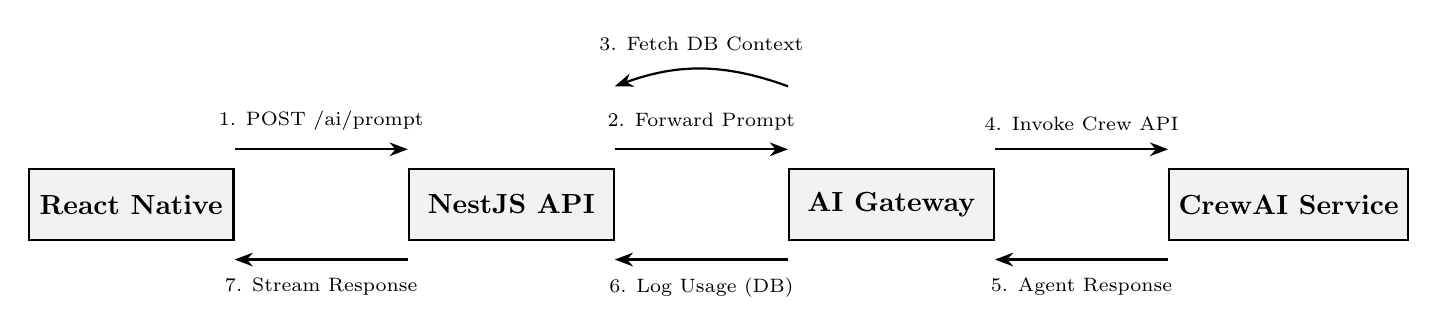
\begin{tikzpicture}[node distance=2.2cm, auto, >=Stealth]
    \tikzstyle{actor} = [rectangle, draw=black, fill=gray!10, thick, minimum width=2.6cm, minimum height=0.9cm, align=center]
    
    \node (client) [actor] {\textbf{React Native}};
    \node (nest) [actor, right=2.2cm of client] {\textbf{NestJS API}};
    \node (gw) [actor, right=2.2cm of nest] {\textbf{AI Gateway}};
    \node (crew) [actor, right=2.2cm of gw] {\textbf{CrewAI Service}};

    % Top Arrows (Shifted cleanly above box top edges)
    \draw[->, thick] ([yshift=0.7cm]client.east) -- node[above=3pt, font=\scriptsize] {1. POST /ai/prompt} ([yshift=0.7cm]nest.west);
    \draw[->, thick] ([yshift=0.7cm]nest.east) -- node[above=3pt, font=\scriptsize] {2. Forward Prompt} ([yshift=0.7cm]gw.west);
    \draw[->, thick] ([yshift=1.5cm]gw.west) to[out=160, in=20] node[above=3pt, font=\scriptsize] {3. Fetch DB Context} ([yshift=1.5cm]nest.east);
    \draw[->, thick] ([yshift=0.7cm]gw.east) -- node[above=3pt, font=\scriptsize] {4. Invoke Crew API} ([yshift=0.7cm]crew.west);

    % Bottom Arrows (Shifted cleanly below box bottom edges)
    \draw[<-, thick] ([yshift=-0.7cm]gw.east) -- node[below=3pt, font=\scriptsize] {5. Agent Response} ([yshift=-0.7cm]crew.west);
    \draw[->, thick] ([yshift=-0.7cm]gw.west) -- node[below=3pt, font=\scriptsize] {6. Log Usage (DB)} ([yshift=-0.7cm]nest.east);
    \draw[<-, thick] ([yshift=-0.7cm]client.east) -- node[below=3pt, font=\scriptsize] {7. Stream Response} ([yshift=-0.7cm]nest.west);
\end{tikzpicture}
}
\caption{AI Gateway and Multi-Agent Sequence Flow Model}
\label{fig:sequence_flow}
\end{figure}

\vspace{1cm}

\section*{Appendix C: To Be Determined List}
Collect a numbered list of the TBD (to be determined) references that remain in the SRS so they can be tracked to closure.

\begin{table}[h!]
\centering
\small
\begin{tabularx}{\textwidth}{|>{\raggedright\arraybackslash}p{2.0cm}|>{\raggedright\arraybackslash}X|>{\raggedright\arraybackslash}p{3.0cm}|>{\raggedright\arraybackslash}p{3.0cm}|}
\hline
\textbf{TBD Item} & \textbf{Description} & \textbf{Target Phase} & \textbf{Owner} \\ \hline
TBD-1 & Benchmark vector embedding performance (1536 vs 3072 dims) under peak load & Phase 2 Testing & Lead Architect \\ \hline
TBD-2 & Evaluate offline local SQLite vector engine for low-connectivity execution & Phase 3 R\&D & Mobile Lead \\ \hline
TBD-3 & Finalize commercial subscription pricing tiers and daily token quotas & Phase 2 Planning & Product Manager \\ \hline
\end{tabularx}
\caption{Numbered List of TBD References}
\end{table}

\end{document}
